\chapter{Konzeptuelle Modellierung und Entwurf}
\label{ch:modellierung}
In diesem Kapitel wird der Anwendungskontext und konkrete Anwendungsfälle nach UCSD sowie Modelle der technischen Umsetzung einer Automatisierungsunterstützung (Informationsmodell, Komponenten-/Dienstemodelle, Architekturmodell) entsprechend RUP modelliert.

\section{User Centered System Design }

Der Anwendungskontext und die Anwendungsfälle werden mithilfe des Ansatzes des User Centered System Design nach \cite{norman1986user} ermittelt. Auf der Grundlage der Anwendungsfälle wird das Informations- und Datenmodell entwickelt und daraus das Komponenten- und Architekturmodell.
Gemäß Aufgabenstellung umfasst die Entwicklung keine graphische Benutzeroberfläche.

\subsection{Anwendungskontext und Anwendungsfälle}

Der Anwendungskontext ist eine Unterstützung bei der Behandlung und Betreuung psychisch erkrankter Personen durch Chatbots. Um den Chatbots den erforderlichen Kontext und das entsprechende Hintergrundwissen zu vermitteln, wird eine Wissensrepräsentation über die psychischen Erkrankungen benötigt. Die zu entwickelnde Konsolenapplikation \emph{MedExtractor} ist dazu gedacht, Forschenden und später auch Chatbots zu ermöglichen, aus einem Input in Form einer reinen Textdatei die Wissensrepräsentation zu erstellen, siehe Abbildung \ref{fig:anwendungsfaelle}. Dazu soll die Applikation mit dem Namen des Textes als Parameter aufgerufen werden. Das Ergebnis der Applikationsausführung ist eine RDF-Datei. 

Als zusätzliche Funktionalität ist denkbar, die Wissensbasis in Form der trainierten spaCy-EntityLinker-Repräsentation auszugeben.


\begin{figure}
    \centering
    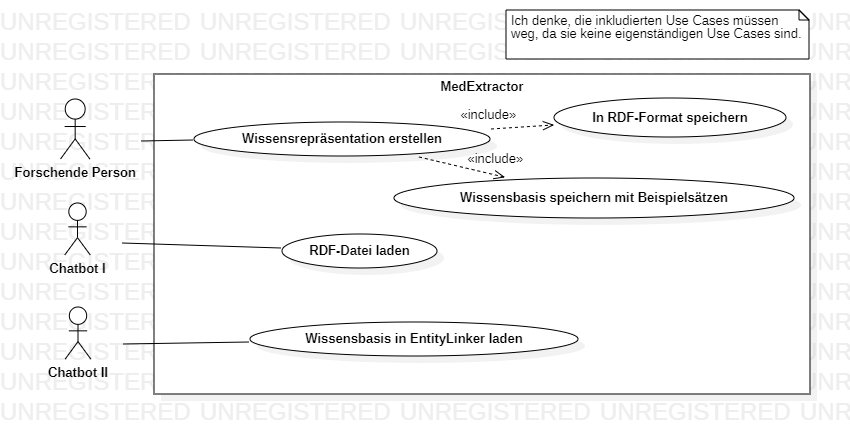
\includegraphics[width=\textwidth]{pictures/UseCases.png}
    \caption{Anwendungsfälle der Konsolenapplikation}
    \label{fig:anwendungsfaelle}
\end{figure}

\subsection{Aktivitätsmodell}

Abbildung \ref{fig:Aktivitätsmodell} stellt das Aktivitätsmodell der Applikation dar.

\begin{figure}[]
    \centering
    \includegraphics[width=\textwidth]{pictures/Aktivitätsdiagramm.png}
    \caption{Aktivitätsdiagramm der Konsolenapplikation}
    \label{fig:Aktivitätsmodell}
\end{figure}

\subsection{Informationsmodell}

Abbildung \ref{fig:informationsmodell} stellt das Informationsmodell der Applikation dar.

\begin{figure}[h]
    \centering
    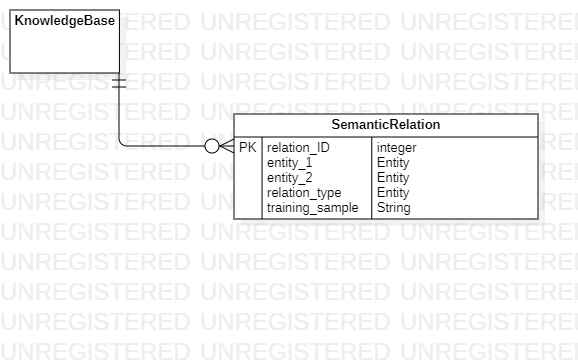
\includegraphics[width=\textwidth]{pictures/Informationsmodell.png}
    \caption{Informationsmodell der Konsolenapplikation}
    \label{fig:informationsmodell}
\end{figure}

\subsection{Komponentenmodell}

Abbildung \ref{fig:komponentendiagramm} stellt das Komponentenmodell der Applikation dar.

\begin{figure}[h]
    \centering
    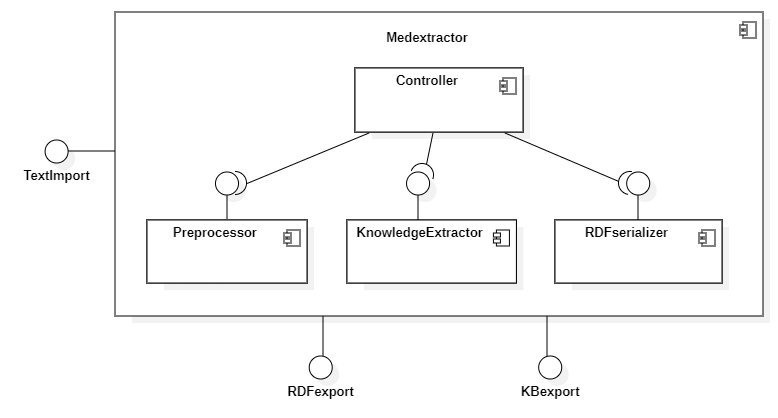
\includegraphics[width=\textwidth]{pictures/ComponentDiagram.png}
    \caption{Komponentenmodell der Konsolenapplikation}
    \label{fig:komponentendiagramm}
\end{figure}

\subsection{Architekturmodell}

Abbildung \ref{fig:architekturmodell} stellt das Architekturmodell der Applikation dar.

\begin{figure}[h]
    \centering
    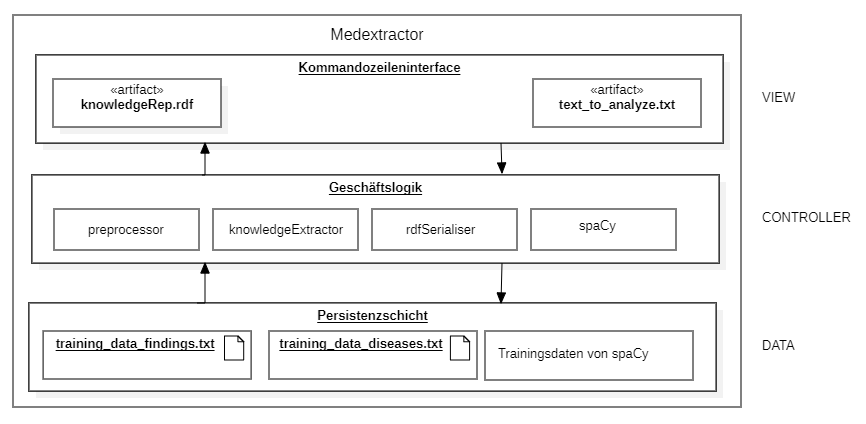
\includegraphics[width=\textwidth]{pictures/Architekturmodell.png}
    \caption{Architekturmodell der Konsolenapplikation}
    \label{fig:architekturmodell}
\end{figure}

Kommandozeileninterface
        |
Geschäftslogik
        |
Gespeicherte Pipeline

\section{FZ 1.2 Theoriebildung zur Vorverarbeitung medizinischer Texte}
\label{sec:FZ1.2} 

Um die Vorverarbeitung medizinischer Texte durchführen zu können, wird dem Präprozessor \ref{fig:preprocessor} der Originaltext übergeben. Umwandlung und Ausgabe des Textes erfolgt über die Methode get\_preprocessed\_text(). Der Text wird in vollständige Sätze umgewandelt, die für sich alleine stehen können. D.h. Aufzählungen werden in Sätze umgewandelt und Pronomen durch konkrete Substantive ersetzt. 
Falls möglich, soll auch eine Indexstruktur (Kapitel-/Abschnittsüberschriften) ermittelt werden.

\begin{figure}[h]
    \centering
    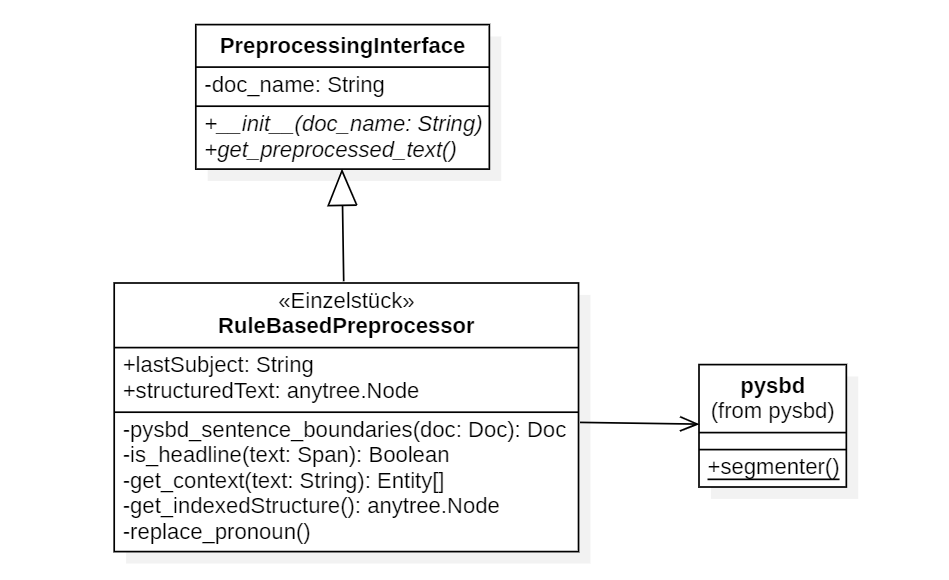
\includegraphics[width=\textwidth]{pictures/RuleBasedPreprocessor.png}
    \caption{Klassendiagramm des Präprozessors der Konsolenapplikation}
    \label{fig:preprocessor}
\end{figure}

\section{FZ 2.3 Theoriebildung zur Überführung medizinischen Fachvokabulars in maschinenlesbare Form zur weiteren Verarbeitung durch NLP}
\label{sec:FZ2.3} 

Beim Starten des MedExtractors wird eine KnowledgeExtractor-Instanz erzeugt (Abbildung \ref{fig:KnowledgeExtractor}). Zur Instanziierung wird der Dateiname der persistent gespeicherten Wissensbasis übergeben. Der EntityRuler wird der spaCy-Pipeline hinzugefügt.

Dieser Instanz kann durch den Aufruf KnowledgeExtractor(text:String) ein vom Preprocessor vorbereiteter \#\#\#Satz\#\#\# zur Analyse übergeben werden. Daher muss KnowledgeExtractor die Methode \_\_call\_\_(text:String) implementieren.

Das KnowledgeExtractor-Objekt verwaltet das KnowledgeBase-Objekt.

Über die Methode set\_context() kann dem KnowledgeExtractor eine Liste von Entitäten übergeben werden (z.B. aus einer Überschrift).

is\_related() ist eine private Methode, die vom KnowledgeExtractor-Objekt verwendet wird, um zu prüfen, ob zwei beliebige vom EntityRuler gefundene Entitäten in Beziehung zueinander stehen. Die SemanticRelation-Objekte werden auf Basis eines wiederholten Aufrufs von is\_related() mit unterschiedlichen Kombinationen gefundener Entitäten erzeugt. 

\begin{figure}[h]
    \centering
    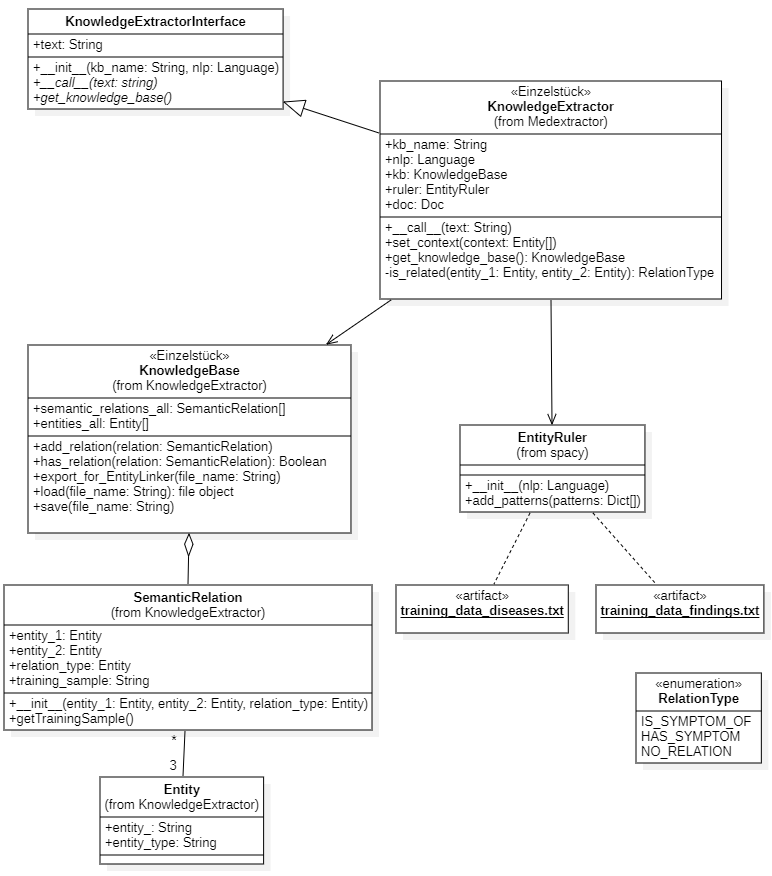
\includegraphics[width=\textwidth]{pictures/KnowledgeExtractor.png}
    \caption{Klassendiagramm des KnowledgeExtractors der Konsolenapplikation}
    \label{fig:KnowledgeExtractor}
\end{figure}

\section{FZ 3.2 Theoriebildung zur Wissensrepräsentation}
\label{sec:FZ3.2} 

Der RdfSerialiser (Abbildung \ref{fig:rdfSerialiser}) serialisiert die Wissensrepräsentation in eine RDF/XML-Datei.

\begin{figure}[h]
    \centering
    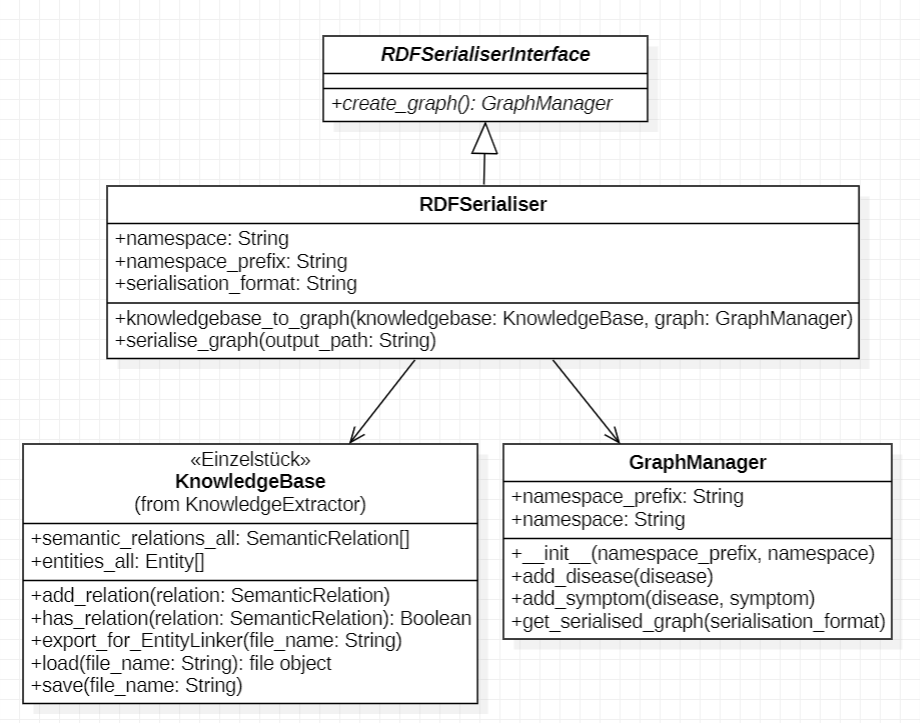
\includegraphics[width=\textwidth]{pictures/RDFSerialiser.png}
    \caption{rdfSerialiser der Konsolenapplikation}
    \label{fig:rdfSerialiser}
\end{figure}



\section{Zusammenfassung}
\label{sec:zusammenfassung modellierung} 

Abbildung \ref{fig:mainClassDiagram} stellt das Hauptklassendiagramm der Applikation dar.

\begin{figure}[h]
    \centering
    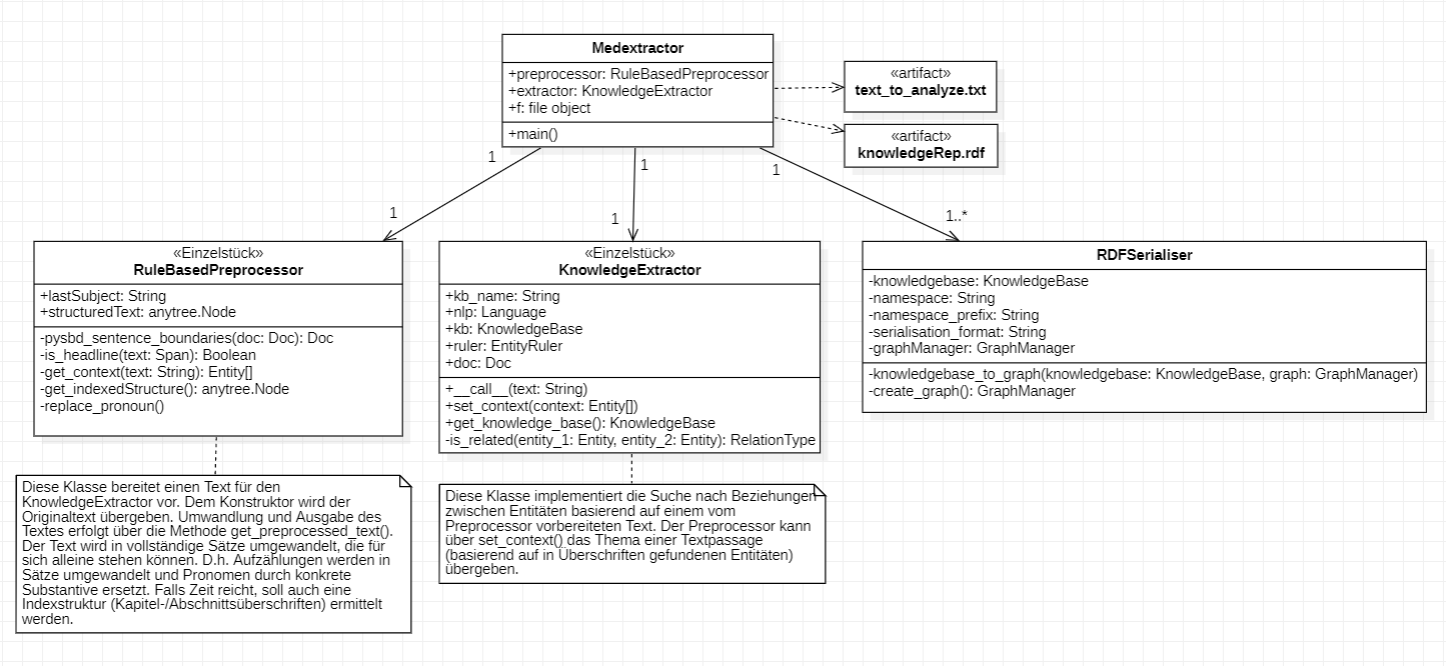
\includegraphics[width=\textwidth]{pictures/Main.png}
    \caption{Hauptklassendiagramm der Konsolenapplikation}
    \label{fig:mainClassDiagram}
\end{figure}